\documentclass[conference]{IEEEtran}
\IEEEoverridecommandlockouts
% The preceding line is only needed to identify funding in the first footnote. If that is unneeded, please comment it out.
\usepackage{cite}
\usepackage{amsmath,amssymb,amsfonts}
\usepackage{algorithmic}
\usepackage{graphicx}
\usepackage{textcomp}
\usepackage{xcolor}
\usepackage{changepage}
\usepackage{ragged2e}
\usepackage[nonumberlist]{glossaries}
\usepackage{url}
\usepackage{lastpage}
\usepackage{fancyhdr}
\usepackage{accents}
\usepackage{blindtext}
\usepackage{hyperref}
\usepackage{algorithm}
\usepackage{gensymb}
\usepackage{enumitem}
\pagestyle{fancy}

\hypersetup
{
    colorlinks=true,
    linkcolor=blue,
    filecolor=magenta,      
    urlcolor=blue,
    citecolor=black,
    pdftitle={Convolutional Coding},
}

\def\BibTeX{{\rm B\kern-.05em{\sc i\kern-.025em b}\kern-.08em
    T\kern-.1667em\lower.7ex\hbox{E}\kern-.125emX}}

\setlength{\parindent}{0pt}
    
\begin{document}

\title{Convolutional Coding
\\
\footnotesize \textsuperscript{*}}

\author{\IEEEauthorblockN{Timothy Holden}
\IEEEauthorblockA{\textit{Department of Electrical and Computer Engineering} \\
\textit{University of Colorado Colorado Springs}\\
Colorado Springs, USA \\
tholden@uccs.edu}}

\maketitle

\begin{abstract}
In communications systems, convolutional coding is a method of error-correcting channel coding which uses parity functions derived from generator configurations to evaluate a specified number of input bits to generate output symbols by sequentially shifting bits into a data stream and evaluating the state of a shift register using an exclusive-or logical operator. In this paper, a code rate of $1/2$ and a constraint length of 9 will be used to simulate the implementation of a convolutional encoding and decoding process of an input message, and measure the effectiveness and accuracy of the implementation based on a variety of metrics such as bit error rate, signal-to-noise ratio, and coding gain.\\
\end{abstract}

\begin{IEEEkeywords}
Encoding, decoding, coding gain, constraint length, code rate, parity functions, generator configuration, Viterbi algorithm, bit error rate, signal-to-noise ratio, most likely path, path metric, exclusive-or
\end{IEEEkeywords}

\section{Introduction}
Since the beginning of time as history portrays it, the progression of communication systems have evolved with mankind. Beginning with cave paintings from the paleolithic era, ancient Sumerian text on stone tablets which led to Babylonian cuniform, smoke signals along the great wall of China to expedite messages, notifications and warnings, ancient Rome's use of carrier pigeons, the use of couriers transporting messages leading to the inception of the postal system, the advent of the newspaper for mass distribution of the written word, and finally to radio-based communications. Radio Frequency (RF) communications was first demonstrated in the late nineteenth century by Nobel Prize Laureate, Guglielmo Marconi for which he referred to as telegraphy without wires. Though Marconi was the first to demonstrate the use of RF communications, it was made possible by Heinrich Hertzs' proof of the existence of radio waves, which was a derivative of James Clerk Maxwell's theory of electromagnetic (EM) radiation describing electricity, magnetism and light as different manifestations of the same phenomenon in 1873.\\

The development of the use of radio waves to transmit and receive information had an enormous impact on humanity, and in particular wireless communications, moving forward into the twentieth century. From the earliest forms of wireless communications being used to transmit Morse Code, short range walkie-talkies, early terrestrial and space-based satellite communications, to modern day 5G (soon to be 6G) terrestrial, as well as sub-Terahertz and optical satellite communications systems, it is clear the technologies developed as a result of RF communications have evolved exponentially over the last 150 years. However, the evolution of wireless communications was not without issues. One of these issues was the rate and capacity of messages through a wireless medium using radio waves, which led one of the most profound, if not the most profound areas of study in communications, which was Information Theory. The subject was the result of a secondary area of interest by Claude Shannon, who in 1941 was working primarily in cryptography during World War II, and later published the result of his paper titled "A Mathematical Theory of Communication" \cite{b1} in the Bell System Technical Journal in 1948. The topic of this paper is based upon concepts which originate in the study of Information Theory, and more specifically how to encode and decode information through a concept known as error correction while limited by the capacity and data rate of a wireless channel, such as an RF link. 

\section{Error Correcting Code}
While capacity and rate are the most obvious constraints specific to communication systems, the implementation of error correcting codes (ECC) is often overshadowed. However, what good is a message, be it small or large, fast or slow, if the received message cannot be reconstructed from the transmitted message? Error correction is the process detecting errors in the transmitted data, and to correct these errors, so to enable the receiver to reconstruct an accurate interpretation of the original message. Due to a variety of different types of inevitable noise relative to the transmission, these errors cannot be avoided, and thus the creation of error correcting codes were introduced to remedy this prevalent and inevitable issue.\\

Channel coding is a complex process by which we add information to the signal to correct errors, but in contrast, we also use source encoding of the data to remove redundancy from the transmission as well. It is important to note that error correction is the detection and correction of errors in a message, and not the prevention of errors in the message. As previously mentioned, the errors introduced within the message are an inevitability of the noise; therefore, the purpose of error correction code (ECC) is to correct the detected errors prior to transmission, and reverse engineer the process by decoding the message on the receiving end. However, the emphasis of this paper is specifically on ECC, and more specifically on a specific type of ECC known as Colvolutional Coding.

\section{Convolutional Coding}
 Convolutional Coding is a type of ECC which sequentially shifts \textit{k} number of bits from one or more input streams into shift registers of a defined size, and uses parity functions derived from generators that define which bits of the shift register are evaluated during each iteration. During each iteration, a bit (or multiple bits) are shifted into the shift register, and the bits defined by the parity equation(s) are applied to an modulo-2 adder (logical exclusive-or operation) which evaluates the appropriate output. The shifting of the bit(s) from the input stream into the shift registers is why the process is referred to as convolutional. 

 \begin{figure}[h]
\centerline{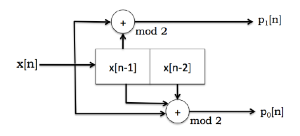
\includegraphics{conv_coder_diagram_300width.png}}
\caption{Block Diagram of Convolutional Encoder}
\label{fig:1}
\end{figure}

 \subsection{Convolutional Coding Parameters}
 Convolutional coding (CC) uses the notation (n,k,K) = (n,k,L), where:\\
 \begin{adjustwidth}{1cm}{0cm}
    n = the \# of output bits\\
    k = the \# of input bits\\
    K = the \# of bits the encoder uses to encode n bits\\
    m = the \# of possible states is $2^{(K-1)}$
 \end{adjustwidth}

 \subsection{Code Rate}
 The code rate (n/k) is the number of bits shifted into the register at every discrete interval divided by the number of bits produced at the output as a result of the coding sequence. The code rate indicates a proportion of input bits and output bits. When a new bit is shifted into the shift register, all other bits shift to the right, with the rightmost bit shifting out of the bit registers. For a code rate of k/n, where $k=1$ and $n=2$, there will be two output bits for each input bit for every iteration/shift. The greater the value of n (output bits) the greater the resilience of bit errors, but the trade-off is that a proportionally higher amount of communications bandwidth is required for coding overhead. 

 \subsection{Constraint Length}
 The constraint length (K) is the number of k-bit shifts that a single bit can influence in the encoder output. Simply put, constraint length is the number of bits that the encoder uses to encode n bits. Typically speaking, the larger the constraint length, the greater resilience to bit errors. The trade-off to improving the resilience to bit errors through the use of a larger constraint length is the increase of required bandwidth for transmission, and the complexity of decoding the encoded message on the receiving end \cite{b2}.\\
 
 Another parameter close associated with the constraint length is the value of \textit{m}, which represents the number of possible states. Given the formula to determine constraint length is $K = m + 1$, where $m$ is equal to the number of memory elements/shift registers (in bytes) needed to represent the state values. The appropriate number of memory elements needed to implement a constraint length of 9, would be $m + 1 =9$. In practice, it is ideal to select the lowest value of \textit{n} and \textit{K} possible while providing a low-enough probability of bit error.

 \subsection{Generator Configuration}
 The polynomial representation of the encoder is based on the Generator configuration (which is conventionally represented in octal form) as a K sized register of the octal values represented in binary format. For example, assume a message sequence of $U = [101101]$, the message polynomial would be as follows:
\begin{equation*}
    U(x) = 1 + x^2 + x^3 + x^5
\end{equation*}
For generator configuration of K=9 configuration, we will use octal formatted values of (453,572), which translates to the following:
\begin{equation*}
    G_1(x) = (453)_8 = [100101011] = 1 + x^3 + x^5 + x^7 + x^8
\end{equation*}
\begin{equation*}
    G_2(x) = (572)_8 = [101111010] = 1 + x^2 + x^3 + x^4 + x^5 + x^7
\end{equation*}
Therefore, to acquire the output polynomial (V), we multiply the message polynomial by each of the generator polynomials as follows:
\begin{equation*}
    V_1(x) = U(x)G_1(x) = (1 + x^2 + x^3 + x^5)(1 + x^3 + x^5 + x^7 + x^8)
\end{equation*}
\begin{equation*}
    V_2(x) = U(x)G_2(x) = (1 + x^2 + x^3 + x^5)(1 + x^2 + x^3 + x^4 + x^5 + x^7)
\end{equation*}
The resulting expansion of both polynomials are as follows:
\begin{equation*}
    V_1(x) = 1 + x^2 + 2x^3 + 3x^5 + x^6 + 2x^7 + 3x^8 + x^9 + 3x^{10} + x^{11} + x^{12} + x^{13}
\end{equation*}
\begin{equation*}
    V_2(x) = 1 + 2x^2 + 2x^3 + 2x^4 + 4x^5 + 2x^6 + 4x^7 + 2x^8 + 2x^9 + 2x^{10} + x^{12}
\end{equation*}
Lastly, the generators derived from the generator polynomials are used to create parity functions to evaluate the bits contained within the shift registers to the bit sequence of the generator. 

\subsection{Parity Equations}
Parity equations are produced by using the total number of encoded data bits within our constraint length (K) of the input stream as the arguments of a generator polynomial $g(x[n], x[n-1], x[n-2], ...)$ which are used to "generate" the parity equations. The number of parity equations is equivalent to the number of output bits (n). Therefore, for a convolutional configuration of (n,k,K) = (2,1,3), we would need two (2) parity equations, which would output two (2) bits for each input (k). For example, if we selected $G_1(1,1,1)$ and $G_2(1,1,0)$, the corresponding polynomial equations would be:
\begin{equation*}
    P_0[n] = x[n] \oplus x[n-1] \oplus x[n-2]
\end{equation*}
\begin{equation*}
    P_1[n] = x[n] \oplus x[n-1]
\end{equation*}

Furthermore, it is important to note that having greater separation between the values of the generator polynomials will provide the best results. This concept alludes to the minimum free distance which is a representation of a convolutional coding configuration for error correction, where higher values represent better error handling relative to the weight of the paths. For example, (1,1,1) of a 3-bit binary sequence would translate to a decimal value of 7, and (1,1,0) of a 3-bit binary sequence would translate to a decimal value of 6. This would imply generator configuration of (7,6) relative to our generator polynomials. If we were to modify the second generator polynomial arguments to (1,0,1), this would translate to a decimal value of 5, which would give us a generator configuration of (7,5) relative to our generator polynomials, which would also provide better results. The following is a more descriptive example of the Convolutional Encoder \cite{b3} comparable to \ref{fig:1} above:
\begin{figure}[h]
\centerline{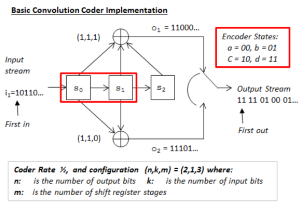
\includegraphics{basic_conv_coder_implementation_300width.png}}
\caption{Basic Convolutional Encoder Implementation}
\label{fig:2}
\end{figure}

\subsection{Convolutional Encoder Transition Table Example}
The following is an example of a transition table having a convolutional configuration of (2,1,3) using generator polynomial configurations of $G_1(1,1,1)$ and $G_2(1,1,0)$ to determine the parity equations used, and the output pair \textit{(n)} for every possible state for an input of 1 or 0 for each state:
\begin{center}
\begin{tabular}{| c | c | c | c |}
 \hline
 \textbf{Input Bit} & \textbf{Input State} & \textbf{Output State} & \textbf{Output Bits} \\ 
 \hline \hline
 $k$ & $S_0 S_1 S_2$ & $S_0 S_1 S_2$ & $n_1 n_2$ \\
 \hline
 0 & 000 & 000 & 00 \\
 \hline
 1 & 000 & 100 & 11 \\
 \hline
 0 & 001 & 000 & 00 \\
 \hline
 1 & 001 & 100 & 11 \\
 \hline
 0 & 010 & 001 & 10 \\
 \hline
 1 & 010 & 101 & 01 \\
 \hline
 0 & 011 & 001 & 10 \\
 \hline
 1 & 011 & 101 & 01 \\
 \hline
 0 & 100 & 010 & 11 \\
 \hline
 1 & 100 & 110 & 00 \\
 \hline
 0 & 101 & 010 & 11 \\
 \hline
 1 & 101 & 110 & 00 \\
 \hline
 0 & 110 & 011 & 01 \\
 \hline
 1 & 110 & 111 & 10 \\
 \hline
 0 & 111 & 011 & 01 \\
 \hline
 1 & 111 & 111 & 10 \\
 \hline
\end{tabular}
\end{center}
It is important to note that when using the $\oplus$ operation on more than two bits, IFF **all of an odd number of bits** are true, the value is returned true (1). In Computer Science this is known as exclusive disjunction, and it is used to determine if there is an odd number of 1 bits, which is the parity bit returned by a parity function (such as in this case).

\section{Convolutional Coding MATLAB Simulation}
The simulation developed for the implementation of a convolutional encoder and decoder for this project was done so using MATLAB 2022b. The convolutional encoder/decoder is using a binary representation of the UTF-8 formatted string "My name is Tim" as the input message. The configuration for convolutional encoder (n,k,K) is as follows:\\
\begin{align*}
    n = 2\\
    k = 1\\
    K = 9\\
\end{align*}
The code rate $k/n = 1/2$ for this configuration with a constraint length \textit{K} of 9, and the normalized signal-to-noise ratio (SNR) $E_b N_o$ (energy per bit to noise power spectral density ratio) is an array of elements from 1 to 10 using a 0.01 step size.\\

Arrays (gen1 \& gen2) have also been created for constraint lengths between 3 and 10  with eight (8) configurations for each to evaluate performance of varying constraint lengths and configurations of the input data. The poly2trellis MATLAB method, which takes the constraint length and the applicable number of generator configurations (two in our case due to $n=2$), was used for encoding and decoding the input message. Upon completion of the encoding and decoding performed by the poly2trellis method, an if-statement was used to determine whether the decoded message was accurate reconstructed. Furthermore, the distspec() method was used to determine the minimum free distance, the bercoding method was used to determine the upper-bound of the BER probability which returns an array of values, the berconfint method was used to calculate the BER based on defined inputs of 1 error in 1,000 trials, at a 95\% confidence interval. Then, the SNR was calculated, and the find method was used to locate the BER index value by which to correlate the two. Lastly, a plot of both the BER against $E_b N_o$ and the BER against SNR are generated upon execution. 

\section{Conclusions}
An analysis was performed for the optimal constraint lengths for 1/2 convolutional codes using the same input message, and methodology described in the \textit{Convolutional Coding MATLAB Simulation} using the generator configurations defined in the following image:
\begin{figure}[h]
\centerline{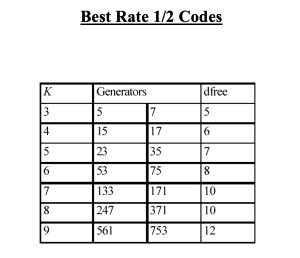
\includegraphics{optimal_constraint_lengths_300width.png}}
\caption{Optimal Generator Configurations for 1/2 Codes}
\label{fig:3}
\end{figure}
The following table demonstrates that as the constraint length was increased, so too did the SNR required to achieve a BER of 0.001 ($10^3$). The coding gain of each varying constraint length when measured as BER against $E_b N_o$ is obvious from the table. Most notably, when $K=9$ is compared to $K=3$ a coding gain of 1.4 dB SNR is achieved. 
\begin{center}
\begin{tabular}{| c | c | c | c |}
 \hline
 \textbf{Constraint Length} & \textbf{Min. Free Dist} & \textbf{BER} & \textbf{SNR} \\ 
 \hline
 9 & 12 & 0.001 & 7.4103 \\
 \hline
 8 & 10 & 0.001 & 7.5103 \\
 \hline
 7 & 10 & 0.001 & 7.9103 \\
 \hline
 6 & 8 & 0.001 & 8.0103 \\
 \hline
 5 & 7 & 0.001 & 8.3103 \\
 \hline
 4 & 6 & 0.001 & 8.6103 \\
 \hline
 3 & 5 & 0.001 & 8.8103 \\
 \hline
\end{tabular}
\end{center}

The calculation of Instructions per Second (MIPS) can be derived similar to that of computer architecture. For the given data rate of 9.6 Kbps, the encoder is taking in the sum of K and n (which in this case would be 11), which is then multipled by the data rate. The bits cancel, and we are left with the number of instructions per second (MIPS). Lastly, we must convert from Kbps to Mbps, which means shifting the decimal three decimal places to the left. This would be represented mathematically as follows:
\begin{center}
$9,600 \dfrac{\text{bits}}{\text{s}}*11\dfrac{\text{instructions}}{\text{bit}}=105,600 \dfrac{\text{instructions}}{\text{s}} \approx 0.105$
\end{center}

The decoder is much more complicated than the encoder and thus requires more instructions. The decoder will ultimately reverse the encoding process, so the number of instructions would be the same of the encoder, in addition to computing the path metric and then finding the most likely path. Therefore, the calculation for Instructions per Second (MIPS) would be represented as follows:
\begin{center}
    $9,600 \dfrac{\text{bits}}{\text{s}}*13\dfrac{\text{instructions}}{\text{bit}}=124,800 \dfrac{\text{instructions}}{\text{s}} \approx 0.125$
\end{center}


Furthermore, when compared to the slides from the lecture on Channel Coding \cite{b5} the theoretical SNR required to achieve a BER of 0.001 with an uncoded system was approximately 10 dB SNR. However, for the simulated system used for this project, the BER at 10 dB SNR was $14*10^{-6}$, and the SNR required for the simulated system was 7.5 dB SNR to achieve a BER of 0.001. 

\subsection{Plots using Varying Constraint Lengths}
The following are a pair of plots of Bit Error Rate Probability against $E_b N0$ and Bit Error Rate Probability against SNR for $K=9$. 
\begin{figure}[!ht]
\centerline{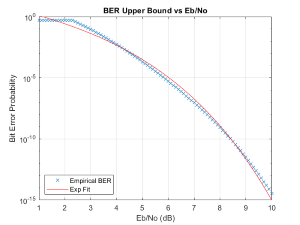
\includegraphics{ber_v_ebno_cl_9_300width.png}}
\caption{Bit Error Rate Probability vs $E_b N_o$}
\label{fig:4}
\end{figure}
\begin{figure}[!ht]
\centerline{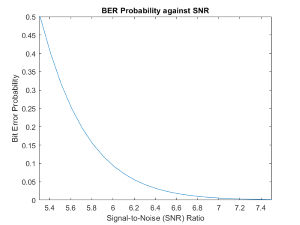
\includegraphics{ber_v_snr_cl_9_300width.png}}
\caption{Bit Error Rate Probability vs SNR}
\label{fig:5}
\end{figure}

\begin{figure}[!ht]
\centerline{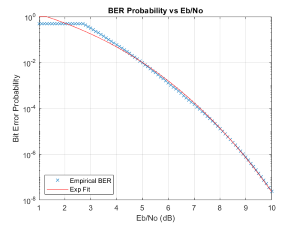
\includegraphics{ber_v_ebno_cl_3_300width.png}}
\caption{Bit Error Rate Probability vs $E_b N_o$}
\label{fig:6}
\end{figure}
\begin{figure}[!ht]
\centerline{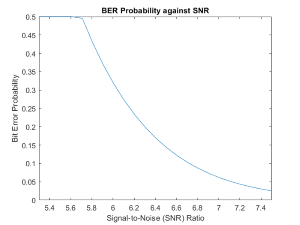
\includegraphics{ber_v_snr_cl_3_300width.png}}
\caption{Bit Error Rate Probability vs SNR}
\label{fig:7}
\end{figure}

\begin{thebibliography}{00}
\bibitem{b1} C. E. Shannon, “A Mathematical Theory of Communication,” The Bell System Technical Journal, vol. 27, pp. 379–423, 623–656, Oct. 1948.
\bibitem{b2} “Lecture 8 Convolutional Encoding,” in MIT 6.02 DRAFT Lecture Notes, 2022.
\bibitem{b3} “A Basic Convolutional Coding Example.” [Online]. Available: https://en.wikibooks.org/wiki/A\_Basic\_Convolutional\_Coding\_Example
\bibitem{b4} [1] R. K. Bansal, S. Bansal, and J. K. Brar, “Goodness Analysis of Generator Polynomial for Convolutional Code with Varying Constraing Length,” IJARCCE, vol. 5, no. 11, 2016, doi: 10.17148/IJARCCE.2016.51174.
\bibitem{b5} [1] M. Frank, “ECE 5965/4965 Introduction to Space Communications: Digital Communications in Space Networks ‘Channel Encoding,’” 2022.


\end{thebibliography}
\end{document}
